\documentclass[fleqn]{article}

%% Created with wxMaxima 23.05.1

\setlength{\parskip}{\medskipamount}
\setlength{\parindent}{0pt}
\usepackage{iftex}
\ifPDFTeX
  % PDFLaTeX or LaTeX 
  \usepackage[utf8]{inputenc}
  \usepackage[T1]{fontenc}
  \DeclareUnicodeCharacter{00B5}{\ensuremath{\mu}}
\else
  %  XeLaTeX or LuaLaTeX
  \usepackage{fontspec}
\fi
\usepackage{graphicx}
\usepackage{color}
\usepackage{amsmath}
\usepackage{grffile}
\usepackage{ifthen}
\newsavebox{\picturebox}
\newlength{\pictureboxwidth}
\newlength{\pictureboxheight}
\newcommand{\includeimage}[1]{
    \savebox{\picturebox}{\includegraphics{#1}}
    \settoheight{\pictureboxheight}{\usebox{\picturebox}}
    \settowidth{\pictureboxwidth}{\usebox{\picturebox}}
    \ifthenelse{\lengthtest{\pictureboxwidth > .95\linewidth}}
    {
        \includegraphics[width=.95\linewidth,height=.80\textheight,keepaspectratio]{#1}
    }
    {
        \ifthenelse{\lengthtest{\pictureboxheight>.80\textheight}}
        {
            \includegraphics[width=.95\linewidth,height=.80\textheight,keepaspectratio]{#1}
            
        }
        {
            \includegraphics{#1}
        }
    }
}
\newlength{\thislabelwidth}
\DeclareMathOperator{\abs}{abs}

\definecolor{labelcolor}{RGB}{100,0,0}

\begin{document}


\noindent
%%%%%%%%
%% INPUT:
\begin{minipage}[t]{4.000000em}\color{red}\bfseries
 --\ensuremath{\ensuremath{>}}	
\end{minipage}
\begin{minipage}[t]{\textwidth}\color{blue}
load(graphs);
\end{minipage}
%%%% OUTPUT:
\[\displaystyle \tag{\% o3} 
\mbox{}
\]"C:/maxima-5.47.0/share/maxima/5.47.0/share/graphs/graphs.mac"



\noindent
%%%%%%%%
%% INPUT:
\begin{minipage}[t]{4.000000em}\color{red}\bfseries
 --\ensuremath{\ensuremath{>}}	
\end{minipage}
\begin{minipage}[t]{\textwidth}\color{blue}
G:\ create\_graph([0,\ 1,\ 2,\ 3,\ 4,\ 5,\ 6],\ \\
\ \ \ \ [[0,\ 2],\ [1,\ 2],\ [2,\ 4],\ [2,\ 3],\ [3,\ 6],\ [4,\ 6],\ [6,\ 5]]);\\
draw\_graph(G,\ prg=circular,fixed\_vertices\ =\ [0,\ 1,\ 2,\ 3,\ 4,\ 5,\ 6],\ show\_id=true,\ redraw=true);
\end{minipage}
%%%% OUTPUT:
\[\displaystyle \tag{G} 
\ensuremath{\mathrm{GRAPH\backslash (7 vertices, 7 edges\backslash )
}}\mbox{}\]

\[\tag{\% t5} 
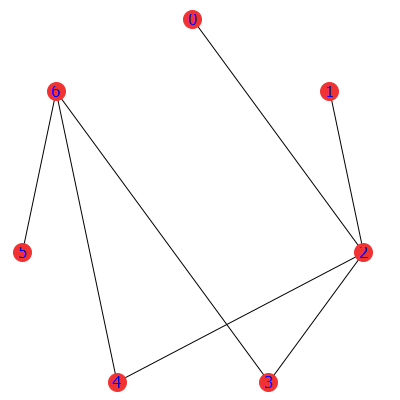
\includegraphics[width=.95\linewidth,height=.80\textheight,keepaspectratio]{graphs_img/graphs_1}\mbox{}\]

\[\tag{\% o5} 
\ensuremath{\mathrm{done}}\mbox{}
\]
%%%%%%%%%%%%%%%%


\noindent
%%%%%%%%
%% INPUT:
\begin{minipage}[t]{4.000000em}\color{red}\bfseries
 --\ensuremath{\ensuremath{>}}	
\end{minipage}
\begin{minipage}[t]{\textwidth}\color{blue}
A:\ minimum\_spanning\_tree(G);\\
draw\_graph(A);
\end{minipage}
%%%% OUTPUT:
\[\displaystyle \tag{A} 
\ensuremath{\mathrm{GRAPH\backslash (7 vertices, 6 edges\backslash )
}}\mbox{}\]

\[\tag{\% t7} 
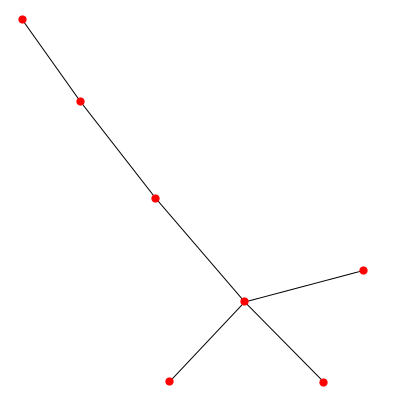
\includegraphics[width=.95\linewidth,height=.80\textheight,keepaspectratio]{graphs_img/graphs_2}\mbox{}\]

\[\tag{\% o7} 
\ensuremath{\mathrm{done}}\mbox{}
\]
%%%%%%%%%%%%%%%%


\noindent
%%%%%%%%
%% INPUT:
\begin{minipage}[t]{4.000000em}\color{red}\bfseries
 --\ensuremath{\ensuremath{>}}	
\end{minipage}
\begin{minipage}[t]{\textwidth}\color{blue}
draw\_graph(G,\ fixed\_vertices\ =\ [0,\ 1,\ 2,\ 3,\ 4,\ 5,\ 6],\ show\_id\ =\ \ true,\ show\_edges=edges(A),\ redraw=true);
\end{minipage}
%%%% OUTPUT:
\[\displaystyle \tag{\% t10} 
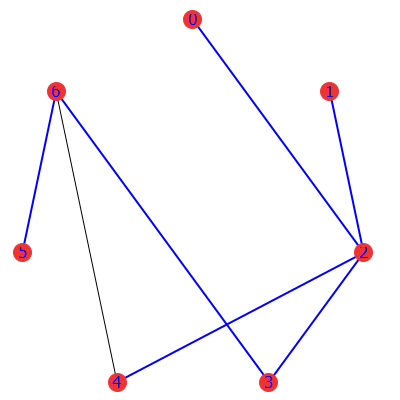
\includegraphics[width=.95\linewidth,height=.80\textheight,keepaspectratio]{graphs_img/graphs_3}\mbox{}\]

\[\tag{\% o10} 
\ensuremath{\mathrm{done}}\mbox{}
\]
%%%%%%%%%%%%%%%%


\noindent
%%%%%%%%
%% INPUT:
\begin{minipage}[t]{4.000000em}\color{red}\bfseries
 --\ensuremath{\ensuremath{>}}	
\end{minipage}
\begin{minipage}[t]{\textwidth}\color{blue}
B:min\_vertex\_cut(G);
\end{minipage}
%%%% OUTPUT:
\[\displaystyle \tag{B} 
[2]\mbox{}
\]
%%%%%%%%%%%%%%%%


\noindent
%%%%%%%%
%% INPUT:
\begin{minipage}[t]{4.000000em}\color{red}\bfseries
 --\ensuremath{\ensuremath{>}}	
\end{minipage}
\begin{minipage}[t]{\textwidth}\color{blue}
draw\_graph(G,\ fixed\_vertices\ =\ [0,\ 1,\ 2,\ 3,\ 4,\ 5,\ 6],\ show\_id\ =\ \ true,\ show\_vertices=B,\ redraw=true);
\end{minipage}
%%%% OUTPUT:
\[\displaystyle \tag{\% t13} 
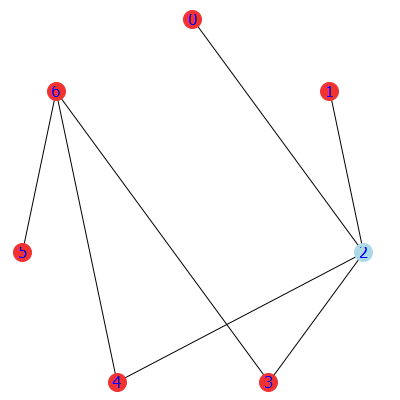
\includegraphics[width=.95\linewidth,height=.80\textheight,keepaspectratio]{graphs_img/graphs_4}\mbox{}\]

\[\tag{\% o13} 
\ensuremath{\mathrm{done}}\mbox{}
\]
%%%%%%%%%%%%%%%%


\noindent
%%%%%%%%
%% INPUT:
\begin{minipage}[t]{4.000000em}\color{red}\bfseries
 --\ensuremath{\ensuremath{>}}	
\end{minipage}
\begin{minipage}[t]{\textwidth}\color{blue}
C:min\_edge\_cut(G);\\
draw\_graph(G,\ fixed\_vertices\ =\ [0,\ 1,\ 2,\ 3,\ 4,\ 5,\ 6],\ show\_id\ =\ \ true,\ show\_edges=C,\ redraw=true);
\end{minipage}
%%%% OUTPUT:
\[\displaystyle \tag{C} 
\left[ \left[ 1\operatorname{,}2\right] \right] \mbox{}\]

\[\tag{\% t15} 
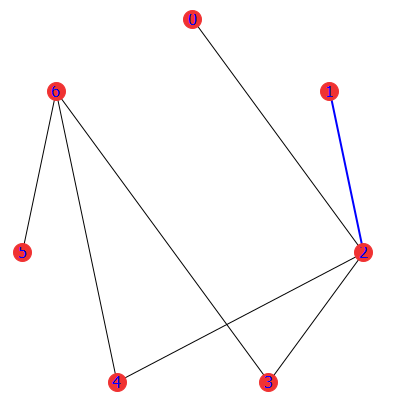
\includegraphics[width=.95\linewidth,height=.80\textheight,keepaspectratio]{graphs_img/graphs_5}\mbox{}\]

\[\tag{\% o15} 
\ensuremath{\mathrm{done}}\mbox{}
\]
%%%%%%%%%%%%%%%%


\noindent
%%%%%%%%
%% INPUT:
\begin{minipage}[t]{4.000000em}\color{red}\bfseries
 --\ensuremath{\ensuremath{>}}	
\end{minipage}
\begin{minipage}[t]{\textwidth}\color{blue}
biconnected\_components(G);
\end{minipage}
%%%% OUTPUT:
\[\displaystyle \tag{\% o16} 
\left[ \left[ 5\operatorname{,}6\right] \operatorname{,}\left[ 1\operatorname{,}2\right] \operatorname{,}\left[ 0\operatorname{,}2\right] \operatorname{,}\left[ 2\operatorname{,}3\operatorname{,}4\operatorname{,}6\right] \right] \mbox{}
\]
%%%%%%%%%%%%%%%%


\noindent
%%%%%%%%
%% INPUT:
\begin{minipage}[t]{4.000000em}\color{red}\bfseries
 --\ensuremath{\ensuremath{>}}	
\end{minipage}
\begin{minipage}[t]{\textwidth}\color{blue}
D:min\_vertex\_cover(G);\\
draw\_graph(G,\ fixed\_vertices\ =\ [0,\ 1,\ 2,\ 3,\ 4,\ 5,\ 6],\ show\_id\ =\ \ true,\ show\_vertices=D,\ redraw=true);
\end{minipage}
%%%% OUTPUT:
\[\displaystyle \tag{D} 
\left[ 2\operatorname{,}6\right] \mbox{}\]

\[\tag{\% t18} 
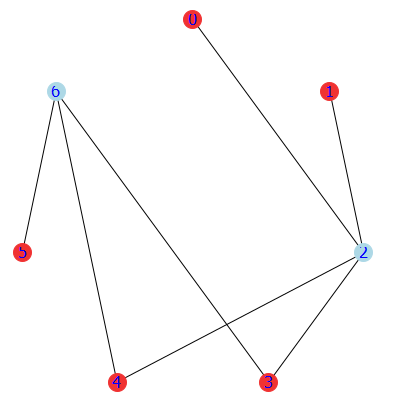
\includegraphics[width=.95\linewidth,height=.80\textheight,keepaspectratio]{graphs_img/graphs_6}\mbox{}\]

\[\tag{\% o18} 
\ensuremath{\mathrm{done}}\mbox{}
\]
%%%%%%%%%%%%%%%%


\noindent
%%%%%%%%
%% INPUT:
\begin{minipage}[t]{4.000000em}\color{red}\bfseries
 --\ensuremath{\ensuremath{>}}	
\end{minipage}
\begin{minipage}[t]{\textwidth}\color{blue}
E:max\_independent\_set(G);\\
draw\_graph(G,\ fixed\_vertices\ =\ [0,\ 1,\ 2,\ 3,\ 4,\ 5,\ 6],\ show\_id\ =\ \ true,\ show\_vertices=E,\ redraw=true);
\end{minipage}
%%%% OUTPUT:
\[\displaystyle \tag{E} 
\left[ 5\operatorname{,}4\operatorname{,}3\operatorname{,}1\operatorname{,}0\right] \mbox{}\]

\[\tag{\% t30} 
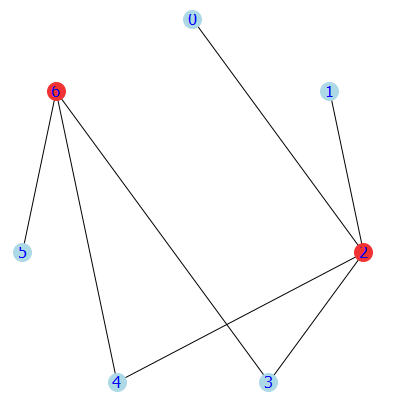
\includegraphics[width=.95\linewidth,height=.80\textheight,keepaspectratio]{graphs_img/graphs_7}\mbox{}\]

\[\tag{\% o30} 
\ensuremath{\mathrm{done}}\mbox{}
\]
%%%%%%%%%%%%%%%%


\noindent
%%%%%%%%
%% INPUT:
\begin{minipage}[t]{4.000000em}\color{red}\bfseries
 --\ensuremath{\ensuremath{>}}	
\end{minipage}
\begin{minipage}[t]{\textwidth}\color{blue}
F:max\_clique(G);
\end{minipage}
%%%% OUTPUT:
\[\displaystyle \tag{F} 
\left[ 0\operatorname{,}2\right] \mbox{}
\]
%%%%%%%%%%%%%%%%


\noindent
%%%%%%%%
%% INPUT:
\begin{minipage}[t]{4.000000em}\color{red}\bfseries
 --\ensuremath{\ensuremath{>}}	
\end{minipage}
\begin{minipage}[t]{\textwidth}\color{blue}
draw\_graph(G,\ fixed\_vertices=[0,\ 1,\ 2,\ 3,\ 4,\ 5,\ 6],\ show\_id=true,\ show\_vertices=F,\ show\_edges=[[0,\ 2]],redraw=true);
\end{minipage}
%%%% OUTPUT:
\[\displaystyle \tag{\% t36} 
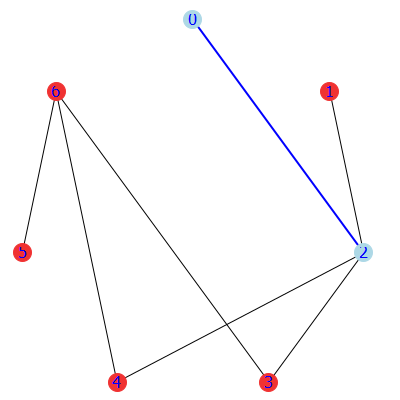
\includegraphics[width=.95\linewidth,height=.80\textheight,keepaspectratio]{graphs_img/graphs_8}\mbox{}\]

\[\tag{\% o36} 
\ensuremath{\mathrm{done}}\mbox{}
\]
%%%%%%%%%%%%%%%%


\noindent
%%%%%%%%
%% INPUT:
\begin{minipage}[t]{4.000000em}\color{red}\bfseries
 --\ensuremath{\ensuremath{>}}	
\end{minipage}
\begin{minipage}[t]{\textwidth}\color{blue}
S:\ random\_bipartite\_graph(6,\ 7,\ 0.75);\\
[A,\ B]\ :\ bipartition(S);\\
draw\_graph(S,\ fixed\_vertices=[0,\ 1,\ 2,\ 3,\ 4,\ 5],\ show\_id=true,\ show\_vertices=A,\ redraw=true);
\end{minipage}
%%%% OUTPUT:
\[\displaystyle \tag{S} 
\ensuremath{\mathrm{GRAPH\backslash (13 vertices, 33 edges\backslash )
}}\mbox{}\]

\[\tag{\% o29} 
\left[ \left[ 2\operatorname{,}4\operatorname{,}3\operatorname{,}1\operatorname{,}0\operatorname{,}5\right] \operatorname{,}\left[ 12\operatorname{,}11\operatorname{,}10\operatorname{,}9\operatorname{,}8\operatorname{,}7\operatorname{,}6\right] \right] \mbox{}\]

\[\tag{\% t30} 
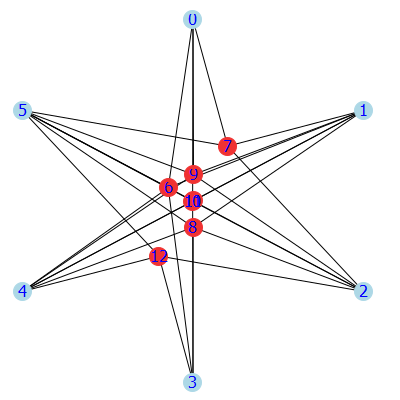
\includegraphics[width=.95\linewidth,height=.80\textheight,keepaspectratio]{graphs_img/graphs_9}\mbox{}\]

\[\tag{\% o30} 
\ensuremath{\mathrm{done}}\mbox{}
\]
%%%%%%%%%%%%%%%%


\noindent
%%%%%%%%
%% INPUT:
\begin{minipage}[t]{4.000000em}\color{red}\bfseries
 --\ensuremath{\ensuremath{>}}	
\end{minipage}
\begin{minipage}[t]{\textwidth}\color{blue}
M:\ max\_matching(S);
\end{minipage}
%%%% OUTPUT:
\[\displaystyle \tag{M} 
\left[ \left[ 0\operatorname{,}7\right] \operatorname{,}\left[ 1\operatorname{,}8\right] \operatorname{,}\left[ 2\operatorname{,}9\right] \operatorname{,}\left[ 3\operatorname{,}10\right] \operatorname{,}\left[ 4\operatorname{,}11\right] \operatorname{,}\left[ 5\operatorname{,}12\right] \right] \mbox{}
\]
%%%%%%%%%%%%%%%%


\noindent
%%%%%%%%
%% INPUT:
\begin{minipage}[t]{4.000000em}\color{red}\bfseries
 --\ensuremath{\ensuremath{>}}	
\end{minipage}
\begin{minipage}[t]{\textwidth}\color{blue}
draw\_graph(S,\ fixed\_vertices\ =\ [0,\ 1,\ 2,\ 3,\ 4,\ 5],\ show\_id\ =\ \ true,\ show\_edges=M,\ show\_vertices=A,\ redraw=true);
\end{minipage}
%%%% OUTPUT:
\[\displaystyle \tag{\% t34} 
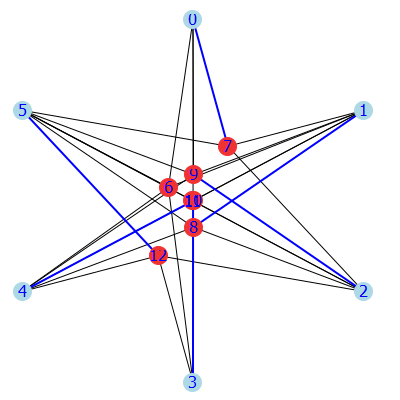
\includegraphics[width=.95\linewidth,height=.80\textheight,keepaspectratio]{graphs_img/graphs_10}\mbox{}\]

\[\tag{\% o34} 
\ensuremath{\mathrm{done}}\mbox{}
\]
%%%%%%%%%%%%%%%%


\noindent
%%%%%%%%
%% INPUT:
\begin{minipage}[t]{4.000000em}\color{red}\bfseries
 --\ensuremath{\ensuremath{>}}	
\end{minipage}
\begin{minipage}[t]{\textwidth}\color{blue}
G\_copy:\ copy\_graph(G);
\end{minipage}
%%%% OUTPUT:
\[\displaystyle \tag{G\_ copy} 
\ensuremath{\mathrm{GRAPH\backslash (7 vertices, 7 edges\backslash )}}\mbox{}
\]
%%%%%%%%%%%%%%%%


\noindent
%%%%%%%%
%% INPUT:
\begin{minipage}[t]{4.000000em}\color{red}\bfseries
 --\ensuremath{\ensuremath{>}}	
\end{minipage}
\begin{minipage}[t]{\textwidth}\color{blue}
for\ edge\ in\ edges(G\_copy)\ do\\
set\_edge\_weight(edge,\ 1+random(15),\ G\_copy);
\end{minipage}
%%%% OUTPUT:
\[\displaystyle \tag{\% o37} 
\ensuremath{\mathrm{done}}\mbox{}
\]
%%%%%%%%%%%%%%%%


\noindent
%%%%%%%%
%% INPUT:
\begin{minipage}[t]{4.000000em}\color{red}\bfseries
 --\ensuremath{\ensuremath{>}}	
\end{minipage}
\begin{minipage}[t]{\textwidth}\color{blue}
shortest\_weighted\_path(0,\ 5,\ G\_copy);
\end{minipage}
%%%% OUTPUT:
\[\displaystyle \tag{\% o39} 
\left[ 29\operatorname{,}\left[ 0\operatorname{,}2\operatorname{,}3\operatorname{,}6\operatorname{,}5\right] \right] \mbox{}
\]
%%%%%%%%%%%%%%%%


\noindent
%%%%%%%%
%% INPUT:
\begin{minipage}[t]{4.000000em}\color{red}\bfseries
 --\ensuremath{\ensuremath{>}}	
\end{minipage}
\begin{minipage}[t]{\textwidth}\color{blue}
swp:\ [[0,2],\ [2,3],\ [3,6],\ [6,5]];
\end{minipage}
%%%% OUTPUT:
\[\displaystyle \tag{swp} 
\left[ \left[ 0\operatorname{,}2\right] \operatorname{,}\left[ 2\operatorname{,}3\right] \operatorname{,}\left[ 3\operatorname{,}6\right] \operatorname{,}\left[ 6\operatorname{,}5\right] \right] \mbox{}
\]
%%%%%%%%%%%%%%%%


\noindent
%%%%%%%%
%% INPUT:
\begin{minipage}[t]{4.000000em}\color{red}\bfseries
 --\ensuremath{\ensuremath{>}}	
\end{minipage}
\begin{minipage}[t]{\textwidth}\color{blue}
draw\_graph(G\_copy\ \ ,\ show\_id=true,\\
label\_alignment=center,\ \ fixed\_vertices=[0,1,2,3,4,5],\ show\_weight=true,\\
vertex\_color=red,\ edge\_color=yellow,\\
show\_edges=swp,\ show\_edge\_color=green);
\end{minipage}
%%%% OUTPUT:
\[\displaystyle \tag{\% t42} 
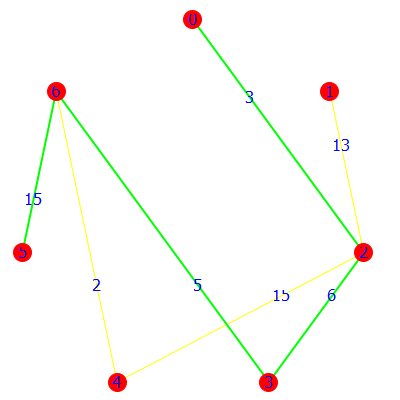
\includegraphics[width=.95\linewidth,height=.80\textheight,keepaspectratio]{graphs_img/graphs_11}\mbox{}\]

\[\tag{\% o42} 
\ensuremath{\mathrm{done}}\mbox{}
\]
%%%%%%%%%%%%%%%%


\noindent
%%%%%%%%
%% INPUT:
\begin{minipage}[t]{4.000000em}\color{red}\bfseries
 --\ensuremath{\ensuremath{>}}	
\end{minipage}
\begin{minipage}[t]{\textwidth}\color{blue}
G4:\ create\_graph([0,1,2,3,4,5,6,7,8,9,10,11,12,13],\\
\ \ \ \ [[[0,\ 1],\ 20],\ [[0,\ 3],\ 15],\ [[0,\ 2],\ 10],[[1,\ 4],\ 15],\ [[1,\ 3],\ 5],\\
\ \ \ \ \ \ \ \ [[2,\ 3],\ 6],\ [[2,\ 5],\ 8],\ [[3,\ 4],\ 4],\ [[3,\ 6],\ 8],\ [[3,\ 5],\ 8],\ [[4,\ 6],\ 9],\ \\
\ \ \ \ \ \ \ \ [[4,\ 7],\ 8],\ [[5,\ 8],\ 16],\ [[5,\ 9],\ 9],\ [[6,\ 5],\ 7],\ [[6,\ 7],\ 12],\ [[7,\ 11],\ 12],\ [[7,\ 10],\ 2],\\
\ \ \ \ \ \ \ \ [[8,\ 7],\ 3],\ [[8,\ 10],\ 9],\ [[8,\ 9],\ 4],\ [[9,\ 12],\ 10],\ [[10,\ 9],\ 5],\ [[10,\ 11],\ 5],\ [[10,\ 13],\ 12],\\
\ \ \ \ [[10,\ 12],\ 6],\ [[11,\ 13],\ 14],\ [[12,\ 13],\ 12]],\\
\ \ \ \ directed=true);
\end{minipage}
%%%% OUTPUT:
\[\displaystyle \tag{G4} 
\ensuremath{\mathrm{DIGRAPH\backslash (14 vertices, 28 arcs\backslash )}}\mbox{}
\]
%%%%%%%%%%%%%%%%


\noindent
%%%%%%%%
%% INPUT:
\begin{minipage}[t]{4.000000em}\color{red}\bfseries
 --\ensuremath{\ensuremath{>}}	
\end{minipage}
\begin{minipage}[t]{\textwidth}\color{blue}
draw\_graph(G4,show\_id=true,\\
label\_alignment=center,fixed\_vertices=[0,1,4,7,11,13,12,9,5,2],show\_weight=true,\\
vertex\_color=gray,edge\_color=red);
\end{minipage}
%%%% OUTPUT:
\[\displaystyle \tag{\% t46} 
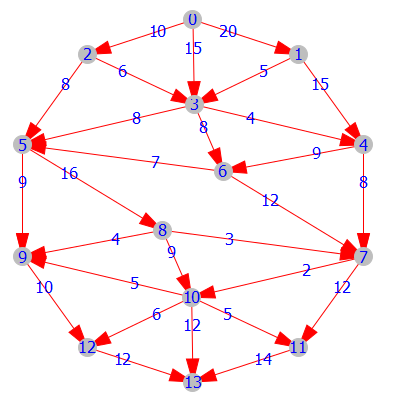
\includegraphics[width=.95\linewidth,height=.80\textheight,keepaspectratio]{graphs_img/graphs_12}\mbox{}\]

\[\tag{\% o46} 
\ensuremath{\mathrm{done}}\mbox{}
\]
%%%%%%%%%%%%%%%%


\noindent
%%%%%%%%
%% INPUT:
\begin{minipage}[t]{4.000000em}\color{red}\bfseries
 --\ensuremath{\ensuremath{>}}	
\end{minipage}
\begin{minipage}[t]{\textwidth}\color{blue}
max\_flow(G4,\ 0,\ 13);
\end{minipage}
%%%% OUTPUT:
\[\displaystyle \tag{\% o47} 
\operatorname{[}33\operatorname{,}\operatorname{[}\left[ \left[ 0\operatorname{,}1\right] \operatorname{,}15\right] \operatorname{,}\left[ \left[ 0\operatorname{,}3\right] \operatorname{,}14\right] \operatorname{,}\left[ \left[ 0\operatorname{,}2\right] \operatorname{,}4\right] \operatorname{,}\left[ \left[ 1\operatorname{,}4\right] \operatorname{,}15\right] \operatorname{,}\left[ \left[ 1\operatorname{,}3\right] \operatorname{,}0\right] \operatorname{,}\left[ \left[ 2\operatorname{,}3\right] \operatorname{,}0\right] \operatorname{,}\left[ \left[ 2\operatorname{,}5\right] \operatorname{,}4\right] \operatorname{,}\left[ \left[ 3\operatorname{,}4\right] \operatorname{,}0\right] \operatorname{,}\left[ \left[ 3\operatorname{,}6\right] \operatorname{,}6\right] \operatorname{,}\left[ \left[ 3\operatorname{,}5\right] \operatorname{,}8\right] \operatorname{,}\left[ \left[ 4\operatorname{,}6\right] \operatorname{,}7\right] \operatorname{,}\left[ \left[ 4\operatorname{,}7\right] \operatorname{,}8\right] \operatorname{,}\left[ \left[ 5\operatorname{,}8\right] \operatorname{,}10\right] \operatorname{,}\left[ \left[ 5\operatorname{,}9\right] \operatorname{,}9\right] \operatorname{,}\left[ \left[ 6\operatorname{,}5\right] \operatorname{,}7\right] \operatorname{,}\left[ \left[ 6\operatorname{,}7\right] \operatorname{,}6\right] \operatorname{,
}\left[ \left[ 7\operatorname{,}11\right] \operatorname{,}12\right] \operatorname{,}\left[ \left[ 7\operatorname{,}10\right] \operatorname{,}2\right] \operatorname{,}\left[ \left[ 8\operatorname{,}7\right] \operatorname{,}0\right] \operatorname{,}\left[ \left[ 8\operatorname{,}10\right] \operatorname{,}9\right] \operatorname{,}\left[ \left[ 8\operatorname{,}9\right] \operatorname{,}1\right] \operatorname{,}\left[ \left[ 9\operatorname{,}12\right] \operatorname{,}10\right] \operatorname{,}\left[ \left[ 10\operatorname{,}9\right] \operatorname{,}0\right] \operatorname{,}\left[ \left[ 10\operatorname{,}11\right] \operatorname{,}0\right] \operatorname{,}\left[ \left[ 10\operatorname{,}13\right] \operatorname{,}11\right] \operatorname{,}\left[ \left[ 10\operatorname{,}12\right] \operatorname{,}0\right] \operatorname{,}\left[ \left[ 11\operatorname{,}13\right] \operatorname{,}12\right] \operatorname{,}\left[ \left[ 12\operatorname{,}13\right] \operatorname{,}10\right] \operatorname{]}\operatorname{]}\mbox{}
\]
%%%%%%%%%%%%%%%%
\end{document}
